\documentclass[11pt,letterpaper]{article}
\PassOptionsToPackage{hyphens}{url}
\usepackage[margin=.83in,top=.8in,bottom=.8in,headheight=15pt]{geometry}
\usepackage[T1]{fontenc}
\usepackage{lmodern,amsmath,amssymb,mathtools,bm,booktabs,array,graphicx,tikz}
\usetikzlibrary{arrows.meta,positioning,calc,decorations.pathreplacing,patterns}
\definecolor{ink}{HTML}{17344D}\definecolor{accent}{HTML}{087E8B}\definecolor{pale}{HTML}{EDF5F5}\definecolor{gold}{HTML}{AD6B19}
\providecommand{\dd}{\,\mathrm{d}}\providecommand{\R}{\mathbb{R}}
\providecommand{\E}{\mathbb{E}}\providecommand{\Var}{\operatorname{Var}}
\providecommand{\Cov}{\operatorname{Cov}}\providecommand{\diag}{\operatorname{diag}}
\providecommand{\norm}[1]{\left\lVert#1\right\rVert}
\providecommand{\abs}[1]{\left|#1\right|}
\usepackage{microtype,hyperref,fancyhdr,enumitem,amsthm,sectsty,needspace}
\allsectionsfont{\raggedright}
\hypersetup{colorlinks=true,linkcolor=ink,urlcolor=accent,pdfauthor={Zan Ahmad},pdftitle={Python and sampled measurements / Lecture notes}}
\setlength{\parindent}{0pt}\setlength{\parskip}{6pt}\linespread{1.07}
\setlist{itemsep=3pt,topsep=4pt,leftmargin=*}
\emergencystretch=2em\clubpenalty=10000\widowpenalty=10000
\pagestyle{fancy}\fancyhf{}\fancyhead[L]{\small Scientific Computing in Python}\fancyhead[R]{\small Lecture 1}
\fancyfoot[L]{\footnotesize Zan Ahmad}\fancyfoot[R]{\footnotesize\thepage}\renewcommand{\headrulewidth}{.3pt}
\newtheorem{proposition}{Proposition}\newtheorem{theorem}{Theorem}\newtheorem{lemma}{Lemma}
\theoremstyle{definition}\newtheorem{definition}{Definition}\newtheorem{example}{Example}
\numberwithin{equation}{section}
\begin{document}
{\small\scshape Scientific Computing in Python\hfill Lecture 1}\par\medskip
{\raggedright\hyphenpenalty=10000\exhyphenpenalty=10000\LARGE\bfseries\color{ink} Python and sampled measurements\par}\medskip
{\small Lecture notes}\par\bigskip
We begin with a temperature record. The calculation is elementary, so that we can examine exactly what the program represents: a value, its physical unit, the time at which it was observed, and the operations applied to it. A program is a sequence of state changes. An equation is a relation between mathematical quantities. Learning to distinguish them is the first step in translating a scientific calculation into Python.

\section{Values and assignment}
\hypertarget{note-values-and-assignment}{}\label{note:values-and-assignment}
{\small \href{slides.html\#frame=values-and-assignment\&step=1}{Slides for this section}}\par
A Python name refers to a value. Assignment evaluates the expression on the right and associates the resulting object with the name on the left. It does not create an equation that Python will solve, nor a permanent dependence between names. Integers represent whole numbers exactly within available memory. Floating-point values represent a finite set of real numbers. Strings are text; a quoted numerical label is not a number.

\begin{minipage}{\linewidth}
\begin{verbatim}
a = 4
b = 2*a
a = 7
\end{verbatim}
\end{minipage}

The final values are $a=7$ and $b=8$. The second line was evaluated before the third.

\subsection*{Expression evaluation}
\begin{minipage}{\linewidth}
\begin{verbatim}
x = 3
print(x**2 + 1)  # 10
print((x + 1)**2)  # 16
\end{verbatim}
\end{minipage}

Exponentiation uses \texttt{**}. Parentheses determine which quantity is squared.
\section{Paired observations}
\hypertarget{note-paired-observations}{}\label{note:paired-observations}
{\small \href{slides.html\#frame=paired-observations\&step=1}{Slides for this section}}\par
Write the observations as ordered pairs $(t_i,T_i)$, where the index identifies an observation. The two lists must have equal length and corresponding entries must refer to the same measurement. An increasing time axis is part of the data definition. Python indexing starts at zero, while a negative index counts backward from the end. A list preserves order; it does not attach a physical unit to its entries.

\[
(t_i,T_i)=(0,80),(60,62),(120,48),(180,38),(240,31).
\]
Time is in seconds and temperature in degrees Celsius.

\begin{minipage}{\linewidth}
\begin{verbatim}
time_seconds = [0, 60, 120, 180, 240]
temperature_c = [80, 62, 48, 38, 31]
\end{verbatim}
\end{minipage}

\subsection*{Indexing the endpoints}
\begin{minipage}{\linewidth}
\begin{verbatim}
t0 = time_seconds[0]
t1 = time_seconds[-1]
T0 = temperature_c[0]
T1 = temperature_c[-1]
\end{verbatim}
\end{minipage}

The endpoint calculation uses $(0,80)$ and $(240,31)$. Interior observations remain relevant to the plotted record.
\section{Units and affine changes of scale}
\hypertarget{note-units-and-affine-changes-of-scale}{}\label{note:units-and-affine-changes-of-scale}
{\small \href{slides.html\#frame=units-and-affine-changes-of-scale\&step=1}{Slides for this section}}\par
A number acquires physical meaning through its unit. Converting seconds to minutes divides the numerical value by 60. Converting Celsius to kelvin adds 273.15. The latter is an affine transformation: it changes the origin but preserves temperature differences. More generally, if $y=ax+b$, then $y_j-y_i=a(x_j-x_i)$. The offset cancels; the scale factor remains.

\[
t_{\rm min}=\frac{t_{\rm s}}{60},\qquad T_K=T_C+273.15.
\]

\[
\Delta T_K=(T_{C,1}+273.15)-(T_{C,0}+273.15)=\Delta T_C.
\]

\subsection*{The same change in two units}
\[
\Delta T=31-80=-49\ ^\circ\mathrm C=-49\ \mathrm K.
\]

\[
\Delta t=240\ \mathrm s=4\ \mathrm{min}.
\]
Temperature differences have equal numerical values in Celsius and kelvin. Absolute temperatures do not.
\begin{center}\begin{minipage}{.98\linewidth}\centering
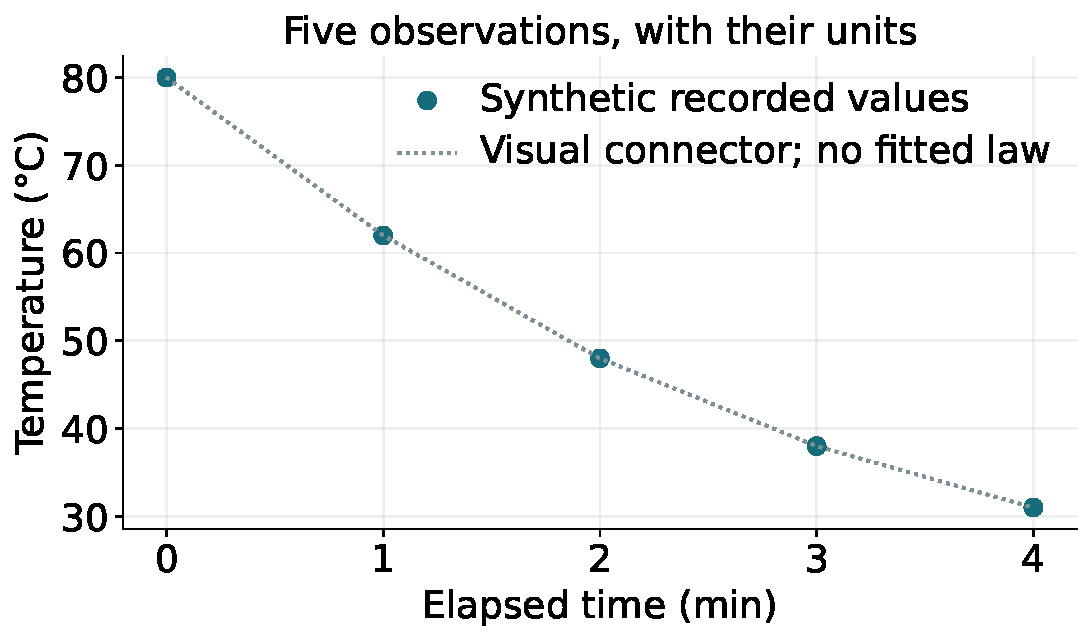
\includegraphics[width=.96\linewidth,height=.57\textheight,keepaspectratio]{presentation-figures/temperature-record.pdf}\par\smallskip
{\small Five supplied observations, with dotted visual connectors only; no continuous cooling law is fitted.}
\end{minipage}\end{center}
\section{Average rate of change}
\hypertarget{note-average-rate-of-change}{}\label{note:average-rate-of-change}
{\small \href{slides.html\#frame=average-rate-of-change\&step=1}{Slides for this section}}\par
The signed average rate is a ratio of differences, not the final temperature divided by elapsed time. It is the slope of the secant through the endpoint observations. A negative value means that the measured quantity decreased over the interval. The unit in the denominator is essential: the numerical rate changes when the time unit changes.

\[
\overline r=\frac{T_1-T_0}{t_1-t_0},\qquad t_1>t_0.
\]

\[
\overline r=\frac{-49}{4}=-12.25\ ^\circ\mathrm C/\mathrm{min}.
\]
This is an interval average, not an instantaneous derivative.

\subsection*{A direct Python calculation}
\begin{minipage}{\linewidth}
\begin{verbatim}
elapsed_min = (time_seconds[-1]-time_seconds[0])/60
change_c = temperature_c[-1]-temperature_c[0]
rate_c_per_min = change_c/elapsed_min
\end{verbatim}
\end{minipage}

A zero elapsed time would make the quotient undefined. The denominator must be checked before division.
\section{Floating-point arithmetic}
\hypertarget{note-floating-point-arithmetic}{}\label{note:floating-point-arithmetic}
{\small \href{slides.html\#frame=floating-point-arithmetic\&step=1}{Slides for this section}}\par
Most decimal fractions do not have a finite binary expansion. Consequently a floating-point calculation usually carries a rounding error, even when the mathematical operation is exact. Equality of integer counters is appropriate; equality of independently computed floating-point expressions often requires a scale-dependent tolerance. A comparison tolerance should be small compared with the physical effect being measured.

\begin{minipage}{\linewidth}
\begin{verbatim}
0.1 + 0.2 == 0.3  # False in binary floating point
\end{verbatim}
\end{minipage}

A useful comparison has the form
\[
|a-b|\leq \varepsilon_{\rm abs}+\varepsilon_{\rm rel}|b|.
\]

\subsection*{Scale in an error tolerance}
The absolute term controls comparisons near zero. The relative term scales with the reference magnitude.

\[
|60r_{\rm s}-r_{\rm min}|\leq 10^{-12}
\]
is a numerical unit-conversion check for this small example. It is not a statement about thermometer accuracy.
\begin{center}\begin{minipage}{.98\linewidth}\centering
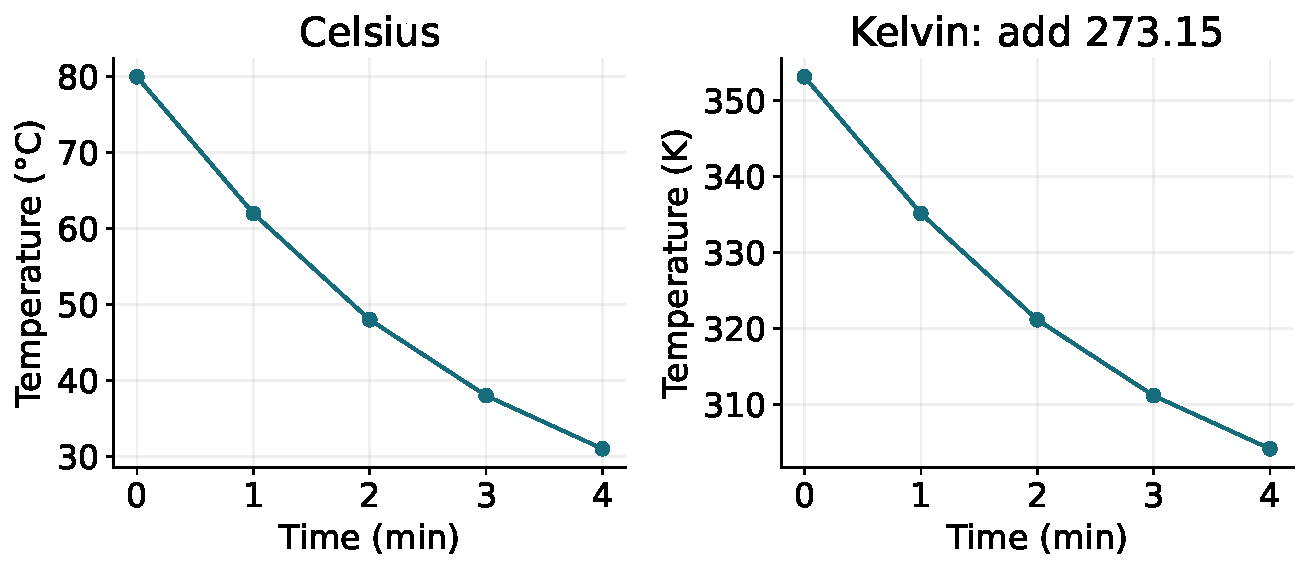
\includegraphics[width=.96\linewidth,height=.57\textheight,keepaspectratio]{temperature-scales.pdf}\par\smallskip
{\small Celsius and kelvin panels represent the same values; adding 273.15 changes absolute numbers while preserving differences.}
\end{minipage}\end{center}
\section{Plots and reproducible execution}
\hypertarget{note-plots-and-reproducible-execution}{}\label{note:plots-and-reproducible-execution}
{\small \href{slides.html\#frame=plots-and-reproducible-execution\&step=1}{Slides for this section}}\par
Plot the pairs $(t_i,T_i)$ with labeled axes. A line segment between observations is a graphical interpolation unless a continuous model has been specified. Restarting a notebook and executing cells in order removes dependence on hidden earlier assignments. The supplied figure helper recreates the documented baseline; editing a separate list does not alter that helper's internal data. Use the editable plotting cell when changing the record.

Five observations determine five plotted points. They do not determine the complete function $T(t)$.

If $g(t_i)=0$ at every sampled time, both $T(t)$ and $T(t)+g(t)$ fit those observations.

\subsection*{A family of indistinguishable interpolants}
For any constant $c$,
\[
g(t)=c\prod_{i=0}^{4}(t-t_i)
\]
vanishes at all five sample times.

Additional assumptions are required to infer behavior between observations.
\bigskip
\section*{Exercises}
\par\noindent\begin{minipage}{\linewidth}
\subsection*{H1-1. Values, text and execution}
New practice; 10 feedback points.

\textbf{a} An experiment records 150 seconds. Convert it to minutes and state the unit cancellation.

\end{minipage}\par\medskip
\textbf{b} x is assigned 150; y is assigned x/60; x is then assigned 240. State y before and after rerunning its assignment.

\textbf{c} Explain why the text value "150" should not be silently treated as a numerical duration. Describe a deliberate correction.

\par\noindent\begin{minipage}{\linewidth}
\subsection*{H1-2. A different temperature record}
Synthetic readings are 50 and 32 degrees Celsius at times 0 and 90 seconds. Total: 10 points.

\textbf{a} Give both temperatures in kelvin.

\end{minipage}\par\medskip
\textbf{b} Compute the endpoint change and average rate in degrees Celsius per minute.

\textbf{c} Must the temperature at 45 seconds be 41 degrees Celsius? Explain.

\par\noindent\begin{minipage}{\linewidth}
\subsection*{H1-3. A plot that someone else can read}
A file contains time\_seconds =\allowbreak{} [0,30,60] and readings\_C =\allowbreak{} [70,55,46]. Total: 10 points.

\textbf{a} State the horizontal values if the plot uses minutes, and write both axis labels.

\end{minipage}\par\medskip
\textbf{b} A colleague changes only the time-axis label from seconds to minutes. Explain the error and a check.

\textbf{c} What goes wrong if the temperature list is reversed while time order stays fixed?

\par\noindent\begin{minipage}{\linewidth}
\subsection*{H1-4. Prepare a reproducible handoff}
A notebook runs only when its author executes cells in a special order. Total: 10 points.

\textbf{a} Give a sequence that makes its dependencies visible.

\end{minipage}\par\medskip
\textbf{b} Describe one execution check and two data checks.

\textbf{c} Write one supported claim and one unresolved question for a two-endpoint temperature record.

\section*{References}
\noindent\begin{minipage}{\linewidth}
Original Python Lecture 0. PDF pages 15--21 and 38--43.

\url{https://zanahmad.com/files/scientific-python/Lecture_0__Intro_to_Python.pdf}
\end{minipage}\par\medskip
Python source materials: Phillip Kerger (2023). Course adaptation and additional exposition: Zan Ahmad.

\end{document}
